\documentclass{beamer}
\usepackage[backend=biber,style=authoryear]{biblatex}

\bibliography{summarize.bib}

% There are many different themes available for Beamer. A comprehensive
% list with examples is given here:
% http://deic.uab.es/~iblanes/beamer_gallery/index_by_theme.html
% You can uncomment the themes below if you would like to use a different
% one:
%\usetheme{AnnArbor}
%\usetheme{Antibes}
%\usetheme{Bergen}
%\usetheme{Berkeley}
%\usetheme{Berlin}
%\usetheme{Boadilla}
%\usetheme{boxes}
%\usetheme{CambridgeUS}
%\usetheme{Copenhagen}
%\usetheme{Darmstadt}
%\usetheme{default}
%\usetheme{Frankfurt}
%\usetheme{Goettingen}
%\usetheme{Hannover}
\usetheme{Ilmenau}
%\usetheme{JuanLesPins}
%\usetheme{Luebeck}
%\usetheme{Madrid}
%\usetheme{Malmoe}
%\usetheme{Marburg}
%\usetheme{Montpellier}
%\usetheme{PaloAlto}
%\usetheme{Pittsburgh}
%\usetheme{Rochester}
%\usetheme{Singapore}
%\usetheme{Szeged}
%\usetheme{Warsaw}

\title{Topic mining for short-text documents on micro-blogging site\\ by combining Doc2Vec and clustering techniques}

\author{Thuong-Hai Pham}
% - Give the names in the same order as the appear in the paper.
% - Use the \inst{?} command only if the authors have different
%   affiliation.

\institute[] % (optional, but mostly needed)
{
 Faculty of Information and Communication Technology\\
 University of Malta\\
 Msida MSD 2080, Malta\\
 Email: thuong-hai.pham.16@um.edu.mt
}
% - Use the \inst command only if there are several affiliations.
% - Keep it simple, no one is interested in your street address.

\date{ICT5901 - Research Methods, 2017}

% the beginning of each subsection:
\AtBeginSubsection[]
{
  \begin{frame}<beamer>{Outline}
    \tableofcontents[currentsection,currentsubsection]
  \end{frame}
}

% Let's get started
\begin{document}

\begin{frame}
  \titlepage
\end{frame}

\begin{frame}{Outline}
  \tableofcontents
  % You might wish to add the option [pausesections]
\end{frame}

\section{Introduction}

\begin{frame}{Introduction}
	\begin{itemize}
		\item Topic model for micro-blogging site
		\item Latent Dirichlet Allocation (LDA)
		\begin{itemize}
			\item state-of-the-art in unsupervised topic model
			\item not trivial task applying directly on short text
		\end{itemize}
		\item LDA Variants
		\begin{itemize}
			\item Author-Topic model
			\item Twitter-LDA
		\end{itemize}
		\item Features learning (doc2vec) \& clustering
	\end{itemize}
\end{frame}

\section{Background}
\subsection{Mathematical background}
\begin{frame}{Mathematical background}
	\begin{block}{Exchangeability}
		$(x_1,x_2...)$ is an infinitely exchangeable sequence of random variables if for any permutation $\pi$,
		\[p(x_1,...,x_n) = p(x_\pi(1),...,x_\pi(n))\]
	\end{block}
	\begin{theorem}{De Finetti, 1935}
		A sequence of random variables $(x_1,x_2,...)$ is infinitely exchangeable iff, for all $n$,
		\[p(x_1,x_2,...,x_n)=\int\prod_{i=1}^{n}p(x_i|\theta)P(d\theta)\]
		for some measure $P$ on $\theta$.
	\end{theorem}
\end{frame}

\subsection{Latent Dirichlet Allocation}
\begin{frame}{Latent Dirichlet Allocation (LDA)}
	\begin{itemize}
		\item Generative probabilistic model
		\item Documents are represented as random mixtures over latent topics
		\item Bag-of-words (BoW) assumption
	\end{itemize}
\end{frame}
\begin{frame}{LDA generative process}
	\begin{figure}[h]
		\centering
		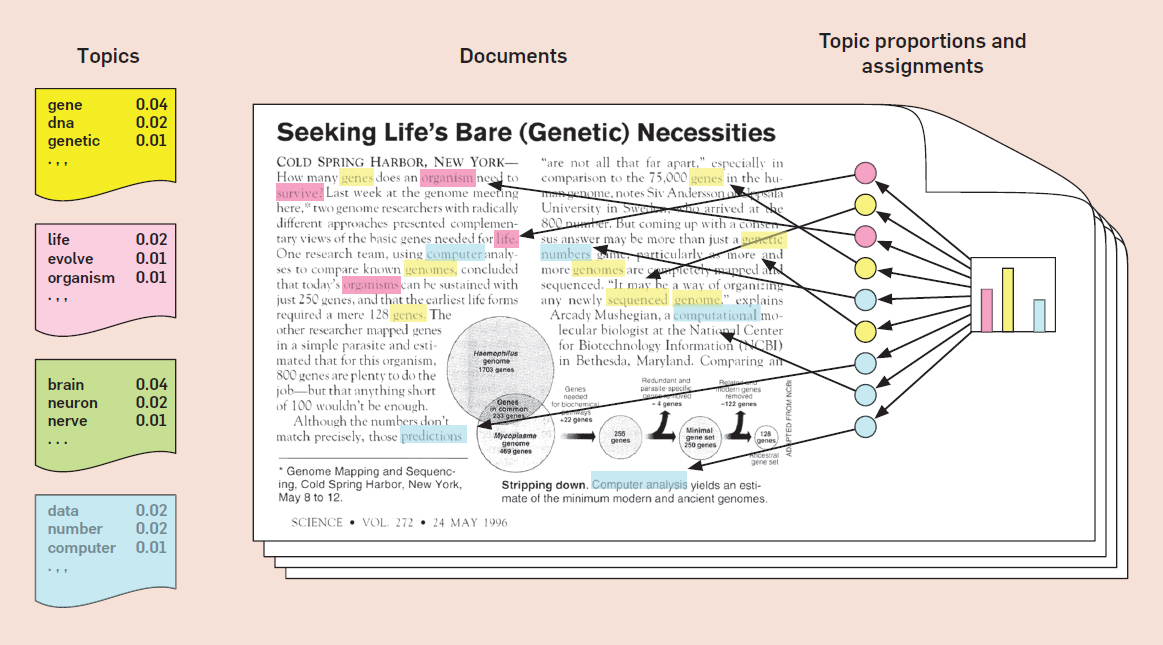
\includegraphics[scale=0.2]{lda_famous}
		\caption{LDA generative process\footnote[frame]{http://cacm.acm.org/magazines/2012/4/147361-probabilistic-topic-models/fulltext}}
	\end{figure}
\end{frame}
\begin{frame}{LDA graphical model}
	\begin{figure}[h]
		\centering
		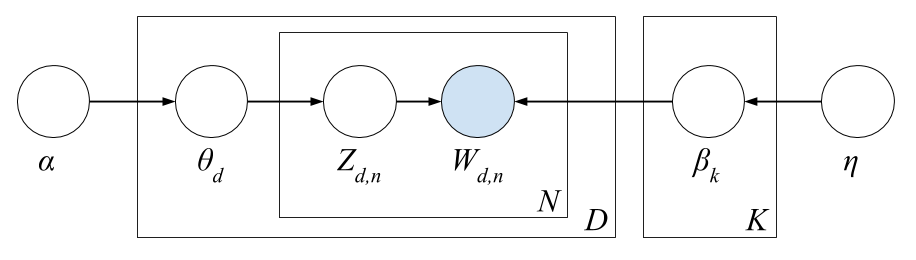
\includegraphics[scale=0.3]{lda_model}
		\caption{LDA graphical model}
		\label{fig:lda_model}
	\end{figure}
\end{frame}

\subsection{LDA variants for Twitter}
\begin{frame}{Author-topic model}
	\begin{itemize}
		\item Excluding the topic proportions for each tweets
		\item Aggregating all tweets of a Twitter's user into a single document \parencite{Weng2010,hong2010empirical}
		\item Efficient on a specific task (e.g. topic-sensitive influencers mining \parencite{Weng2010})
	\end{itemize}
\end{frame}
\begin{frame}{Twitter-LDA}
	\begin{figure}[h]
		\centering
		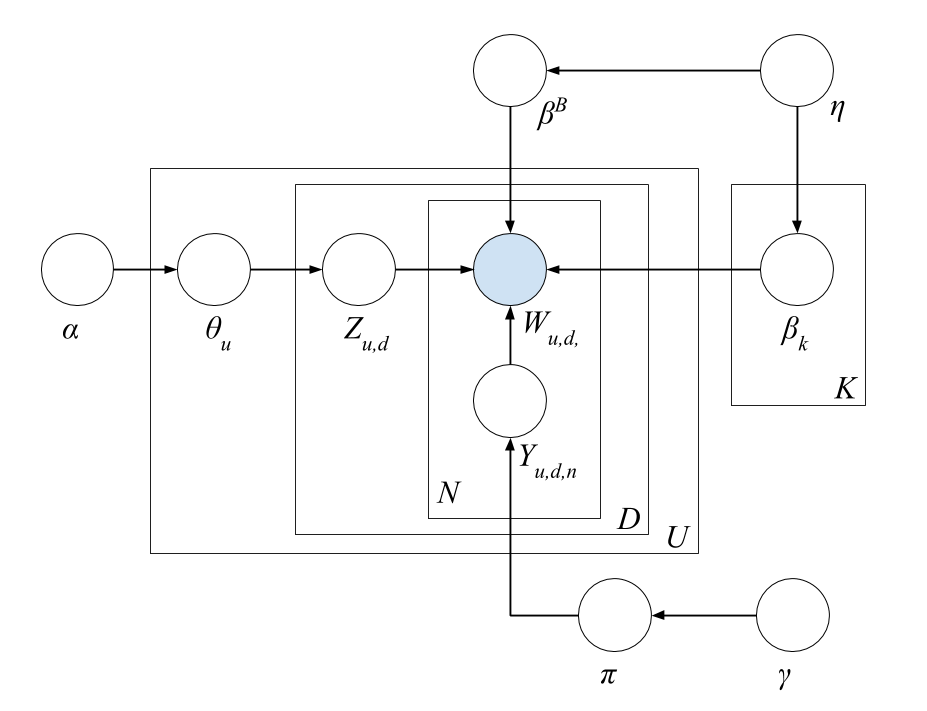
\includegraphics[scale=0.2]{twitter_lda_model}
		\caption{Twitter-LDA graphical model}
		\label{fig:twitter_lda_model}
	\end{figure}
\end{frame}

\subsection{Evaluation}
\begin{frame}{Evaluation}
	\begin{itemize}
		\item Intrinsic: view the problem as document modelling \parencite{Blei2003} by measuring perplexity of held-out set $C'$
		\[perp(C')=exp\left\{-\frac{\sum_{d=1}^{D}{log(p(W_d))}}{\sum_{d=1}^{D}N_d}\right\}\]
		\item Extrinsic: measure LDA performance on some secondary tasks, such as corpus comparison or topic-sensitive influencers mining \parencite{Weng2010}
		\item Human evaluation: human judges assign a score on each topic, ranging from 1 (meaningful) to 0 (nonsense)\parencite{zhao2011comparing}
	\end{itemize}
\end{frame}

\section{Proposed method}
\subsection{Method}
\begin{frame}{Doc2vec as features learning \parencite{le2014distributed}}
	\begin{figure}
		\centering
		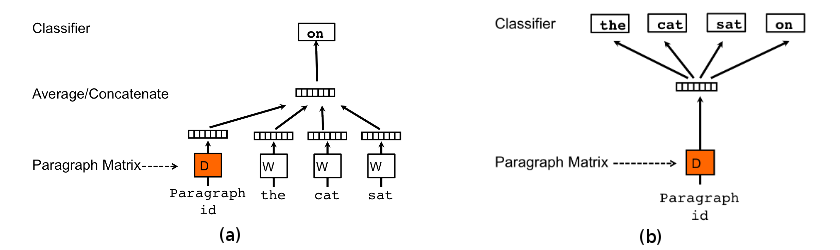
\includegraphics[scale=0.35]{doc2vec_hor}
		\caption{Framework for learning paragraph vector, (a) Distributed Memory, (b) Distributed Bag of Words}
		\label{fig:doc2vec}
	\end{figure}
\end{frame}

\begin{frame}{Clustering}
	\begin{itemize}
		\item K-means: traditional clustering 
		\item DBSCAN: no K specified
		\item C-means: fuzzy/soft clustering
	\end{itemize}
\end{frame}

\begin{frame}{Evaluation}
	\begin{itemize}
		\item Perplexity does not measure how \alert{meaningful} the topics discovered are
		\item Human evaluation strategy \parencite{zhao2011comparing}
		\begin{itemize}
			\item Two distinct judges
			\item Score from 0 to 10 for meaningfulness
			\item Score for mutual agreement on topic assignments
		\end{itemize}
	\end{itemize}
\end{frame}

\subsection{Tasks}
\begin{frame}{Timeline}
	\begin{figure}
		\centering
		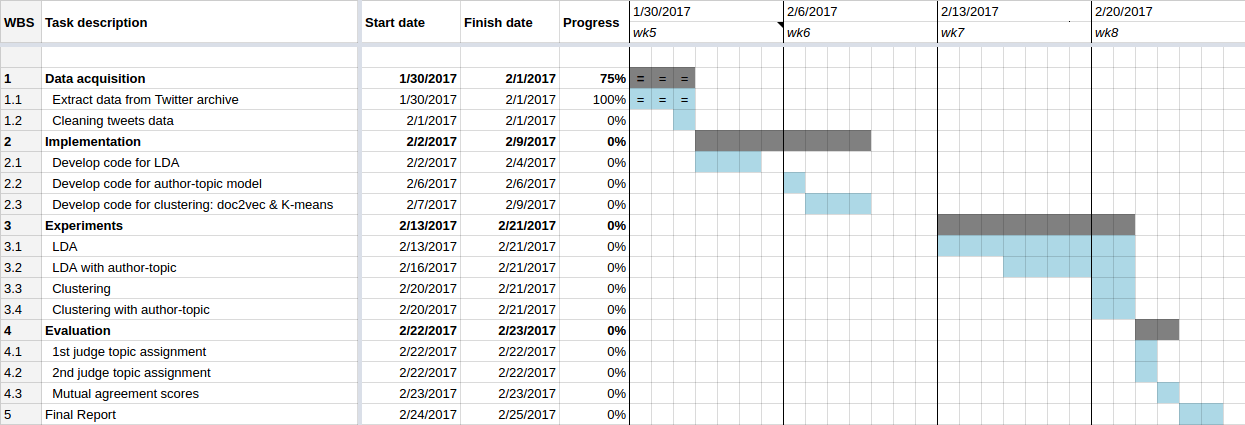
\includegraphics[width=\textwidth]{project_timeline}
		\caption{Project timeline}
		\label{fig:project_timeline}
	\end{figure}
\end{frame}

\begin{frame}{Resources}
\begin{itemize}
	\item Data: Twitter stream archive\footnote[frame]{https://archive.org/details/archiveteam-twitter-stream-2016-07} in July 2016
	\item Compute engine: Google cloud n1-standard-4\footnote[frame]{operates with 4 virtual CPUs, 15GB RAM, 200GB hard disk drive}
	\item Code library: LDA and Doc2Vec model in Gensim\footnote[frame]{https://radimrehurek.com/gensim/} library
	\item Evaluation: 02 human judges
\end{itemize}
\end{frame}

\section{Expected result \& difficulties}
\begin{frame}{Expected result}
	\begin{block}{Meaningfulness}
		Proposed method of combining Doc2Vec and K-means achieves \alert{approximate meaningfulness} score in compare to traditional LDA method
	\end{block}
	\begin{block}{Advantages}
		\begin{itemize}
			\item Eliminate assumptions in LDA variants
			\item Capability of running on short-text documents (social networks)
		\end{itemize}
	\end{block}
\end{frame}
\begin{frame}{Difficulties}
	\begin{itemize}
		\item Noise in unconventional language usage on Twitter
		\item Twitter stream archive is too large to consume at once
		\item Meaning of topics discovered can be unclear or hardly interpretable
	\end{itemize}
\end{frame}

% All of the following is optional and typically not needed. 
\appendix
\section<presentation>*{\appendixname}
\begin{frame}[allowframebreaks]
  \frametitle<presentation>{References}
    
	\printbibliography
\end{frame}

\end{document}


